% Chapter 2

\chapter{Literature Review} % Introduction


\label{Chapter2} % 

Within literature the problem of predicting the next occurence of an event is referred to as event prediction, sequence prediction, or point process modeling. Analyzing data of this sort presents its own unique challenges and questions. What are the ways to represent the data?  What types of stochastic 
models  are  appropriate  for  explaining  the  structure  in  the  data? How  can  we  measure  
how  well  the  data  is  described  by  a  particular  model?  

Regarding the representation of the event data, there are three ways of doing this, event count, event times, and inter-event intervals (see figure \ref{fig:fig1}).

\begin{figure}[h!]
	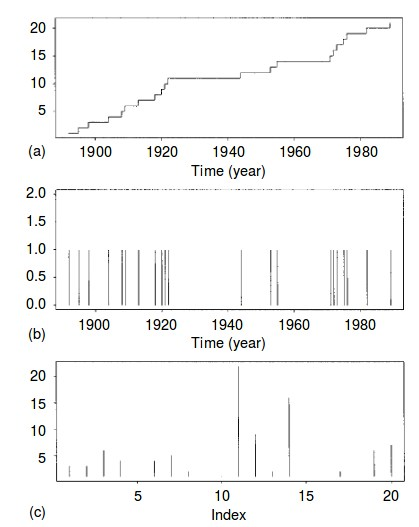
\includegraphics[width=7cm, keepaspectratio]{fig001.jpg}
	\caption{Three different representations of the same point-process a) event count b) date of occurence c) interval time between floods}
	\label{fig:fig1}
\end{figure}

Inter-event has traditionally been one of the most common ways od representing the data, for example in the times between financial transactions \parencite{EngleRusell}.

\section{Poisson Point Process}

Poisson processes \parencite{Kingman} are characterized by the fact that the probability of an event in a small time interval is independent of the event at all other times. 

By making use of this independence assumption one can make sure of models that construct a poisson distribution to describe the data. Due to their ease of use Poisson processes are often the first-order models used to  characterize  spiking  systems. However given the intercorrelation between time intervals they are not so useful for temporal point processes. However in some cases it is possible to aggregate temporal data into a form that removes the inter-dependence between occurrences. We see this in used in the Bayesian Inference model described in the next chapeter.

\section{Temporal Point Processes}

A temporal point process \parencite{DaleyJones} is a way of modeling event data as a sequence of a fixed period intervals. Temporal point processe models seek to estimate the probability of an event happening at time $t$, based on an event history upto, but not including, time $t$.  At its simplest it can be represented as:
$${\xi =\sum _{i=1}^{n}\delta _{X_{i}},}$$

where $\delta$ denotes the Dirac measure, a probability measure of whether a set contains point $X$ or not.

In the case of music listening we can model a sequence of events and non-events, where $t_i$ can either be 0 (did not play music) or 1 (played music). This is the form we use in all but the Bayesian model as described in the next chapter.

\subsection{Conditional Intensity Function in Point Processes}

The conditional intensity function is a key part of traditional point processes modeling in which the probability of an event $\lambda(t)$ is derived from a stochastic model of the inter-event time \parencite{DuWang}, for instance the Poisson process at time $t$.

Conditional intensity functions can be inhomogenous such as with a Gaussian Kernel $\lambda(t) = \sum^k_{i=1}\alpha(2\pi \sigma^2_i)^{-1/2}exp(-(t-c_i)^2/\sigma^2_i)$
, for $t \epsilon [0,T]$ where $c_i$ and $\sigma$ are fixed center and standard deviations, respectively, and $\alpha_i$ is the weight for kernel i.

Or they can vary in intensity, such as with the self-exciting (Hawkes) process where the intensity is determined by previous events through the parametric form $\lambda(t) = \mu + \beta \sum_{t_i<t}g(t-t_i)$ and where $g$ is some non-negative kernel function.

However as noted by Wass et. al \parencite{Wass}, conventional point process models often make unrealistic assumptions about the generative processes of the event sequences. The conditional intensity function make various parametric assumptions about the latent dynamics governing the generation of the observed point patterns. As a consequence, model misspecification can cause significantly degraded performance using point process models.


\section{Deep RNN Point Process Models}

In recent years deep learning has demonstrated the power to learn hierarchical nonlinear patterns on large-scale datasets \parencite{DL} through multiple layers of abstraction (e.g. multi-layer feedforward neural networks). It has achieved state-of-the-art performances on a wide range of applications, such as computer vision \parencite{ImageNet}, natural language processing \parencite{Socher}, and protein structure prediction \parencite{Lena}.

However it has not been applied to temporal point processes until recently with Xiao et. al \parencite{Wass} applying Generative Adversarial Networks (GANS) to the problem. GANs consist of two neural network models - a generator tasked with generating (i.e. predicting) a future sequence of events based on the history, and a discriminator tasked with detecting the true (fround truth) sequence amongst the generated ones.

For measuring the loss between a generated and true sequence, the authors found the Wassertein-Distance \parencite{WassGAN} performed better than Maximum Likihood Estimate (MLE) which they remarked "may suffer from mode dropping or get stuck in an inferior local minimum".

Their findings showed that where as parametric point process models work better with problems where a parametetric form exists, with real world data a GAN model with Wasserterin-Distance outperformed all other models (including an RNN model using MLE). This signals a promising new direction for temporal point process research.

\section{Summary}

While not an exhaustive review of techniques we have seen some of the ways in which point processes can be modelled both traditionally and more recent areas of experiments. Historically a lot of methods have focussed on modeling the data as inter-event times. In the next chapter we will lay out our own methodology for how to structure the data followed by a range methods we wish to assess for modeling the temporal patterns.